\subsection{Energy transducers and Smart metering in railways}

\begin{frame}{Remote Monitoring in Railways}{Energy transducers}

	\begin{block}{\textbf{Transducers}}
	
%	\begin{minipage}[t]{0.48\linewidth}
%		\vspace{5em}
%	\begin{itemize}
%		\item Magnetic Coupling
%		\item Magneto Resistance
%		\item Faraday Induction
%		\item Hall Effect
%	\end{itemize}
%	\end{minipage}\hfill
%	\begin{minipage}[t]{0.48\linewidth}
		%\begin{itemize}
		%	\item  50 Hz 25 kV supply system.
		
		%\end{itemize}
	\begin{minipage}[t]{0.48\linewidth}
		\centering{
		\begin{figure}[ht!]
			\centering
			\vspace{1em}
			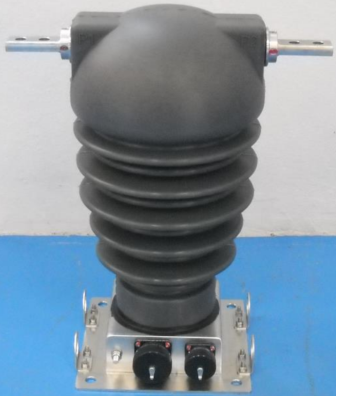
\includegraphics[width=0.45\textwidth,keepaspectratio]{figures/32.EnergyS/current_t}
			\caption{25 kV current transformer. Adapted from \textit{www.railware.it}}
		\end{figure}
	}
	\end{minipage}	
	\begin{minipage}[t]{0.48\linewidth}
	\centering{
			\begin{figure}[ht!]
			\centering
			\vspace{1em}
			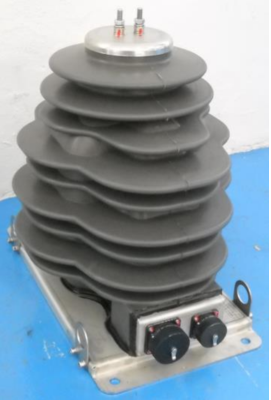
\includegraphics[width=0.35\textwidth,keepaspectratio]{figures/32.EnergyS/voltage_t}
			\caption{25 kV voltage transformer. Adapted from \textit{www.railware.it}}
		\end{figure}
}	
		
	\end{minipage}
	

		
	\end{block}
\end{frame}
%%%%%%%%%%%%%%%%%%%%%%%%%%%%%%%%%%%%%%%%%%%%%%%%%%%%%%%%%%%%%%%%%%%%%%%%%%%%%%%%%%%%%

\begin{frame}{Remote Monitoring in Railways}{Energy transducers --- Power Calculation Function}
%\begin{block}{\textbf{Overview of Existing European Railway Power Systems}}


\begin{figure}[h!]
	\centering
	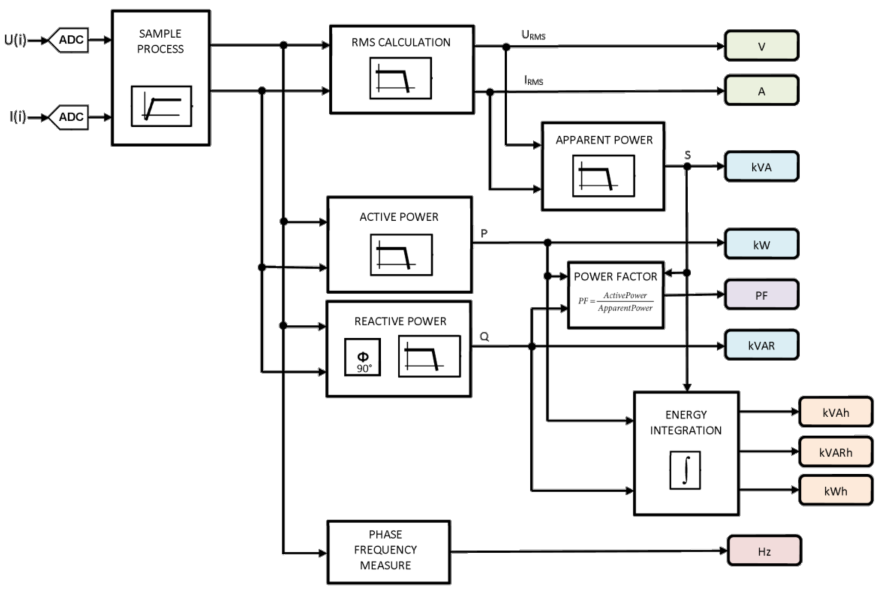
\includegraphics[width=0.7\textwidth,keepaspectratio]{figures/32.EnergyS/energy_calculation}
	\caption{EcoS power calculation function, based on EN50463. Adapted from railware.it}
\end{figure}
	
	
%\end{block}
\end{frame}
%%%%%%%%%%%%%%%%%%%%%%%%%%%%%%%%%%%%%%%%%%%%%%%%%%%%%%%%%%%%%%%%%%%%%%%%%%%%%%%%%%%%%
%\subsection{Smart metering in railways}

\begin{frame}{Remote Monitoring in Railways}{Smart metering in railways}

\begin{figure}[h!]
	\centering
	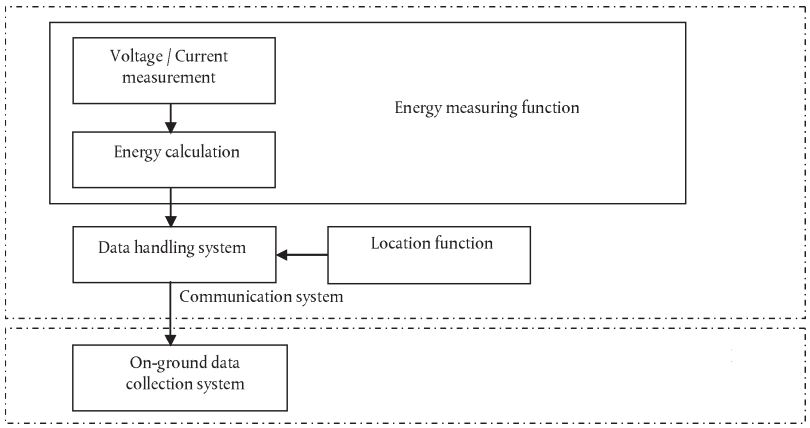
\includegraphics[width=0.8\textwidth,keepaspectratio]{figures/34.SmartM/EMS}
	\caption{Functions, data flow and regulation scope of on-board energy measurement system.}
\end{figure}

\end{frame}
%%%%%%%%%%%%%%%%%%%%%%%%%%%%%%%%%%%%%%%%%%%%%%%%%%%%%%%%%%%%%%%%%%%%%%%%%%%%%%%%%%%%%

\subsection{Wireless Networks and Decision Support Systems}

\begin{frame}{Remote Monitoring in Railways}{Wireless Networks}

\begin{figure}[h!]
	\centering
	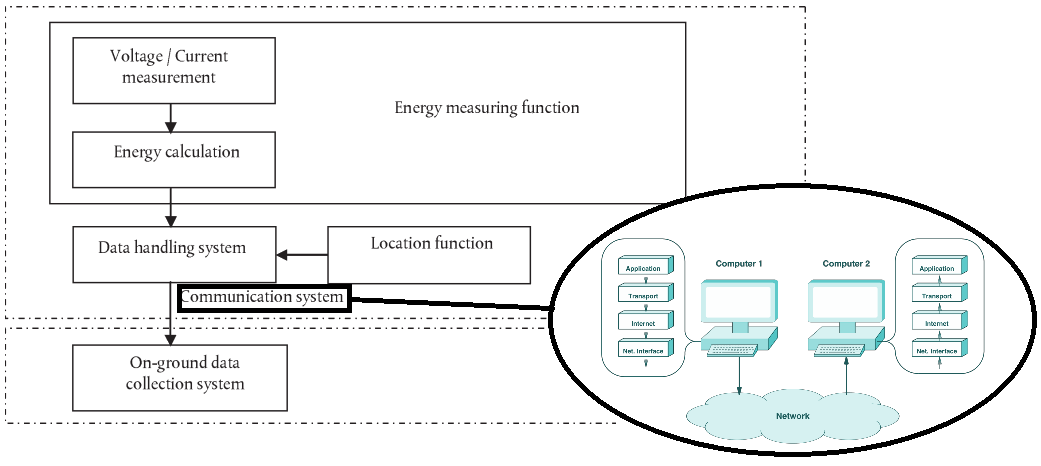
\includegraphics[width=0.8\textwidth,keepaspectratio]{figures/34.SmartM/EMS2}
	\caption{Detail in the communication system: integration with wireless computer networks. Adapted from \cite{comer2008}.}
\end{figure}

\end{frame}
%%%%%%%%%%%%%%%%%%%%%%%%%%%%%%%%%%%%%%%%%%%%%%%%%%%%%%%%%%%%%%%%%%%%%%%%%%%%%%%%%%%%%


\begin{frame}{Remote Monitoring in Railways}{Wireless Networks --- Simulators}
\begin{block}{\textbf{Wireless Networks --- Simulators}}
	
	\begin{minipage}[t]{0.48\linewidth}
	%	\vspace{5em}
		\begin{itemize}
			\item NS-3
			\item OMNeT++
			\item QualNet 7.0 + EXata 5
			\item MatLab + Simulink
		\end{itemize}
	\end{minipage}\hfill
	\begin{minipage}[t]{0.48\linewidth}
		
		\begin{figure}[ht!]
			\centering
			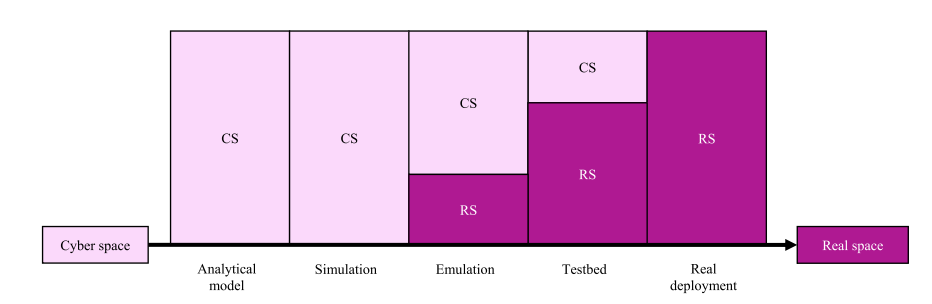
\includegraphics[width=1\textwidth,keepaspectratio]{figures/33.WirelessN/simul_VS_emul}
			\caption{Simulation \& emulation framework.}
		\end{figure}
	
	\end{minipage}
	
	
	
\end{block}
\end{frame}
%%%%%%%%%%%%%%%%%%%%%%%%%%%%%%%%%%%%%%%%%%%%%%%%%%%%%%%%%%%%%%%%%%%%%%%%%%%%%%%%%%%%%

%%%%%%%%%%%%%%%%%%%%%%%%%%%%%%%%%%%%%%%%%%%%%%%%%%%%%%%%%%%%%%%%%%%%%%%%%%%%%%%%%%%%%



%\subsection{Decision Support Systems}
%%%%%%%%%%%%%%%%%%%%%%%%%%%%%%%%%%%%%%%%%%%%%%%%%%%%%%%%%%%%%%%%%%%%%%%%%%%%%%%%%%%%%


%\begin{frame}{Remote Monitoring in Railways}{Decision Support Systems}
%\begin{block}{\textbf{Decision Support Systems}}
	
%	\begin{minipage}[t]{0.48\linewidth}
		%	\vspace{5em}
%		\begin{itemize}
%			\item Eco-driving --- Driving Assistant
%			\item Timetable Scheduling
%		\end{itemize}
%	\end{minipage}\hfill
%	\begin{minipage}[t]{0.48\linewidth}
		
%		\begin{figure}[ht!]
%			\centering
%			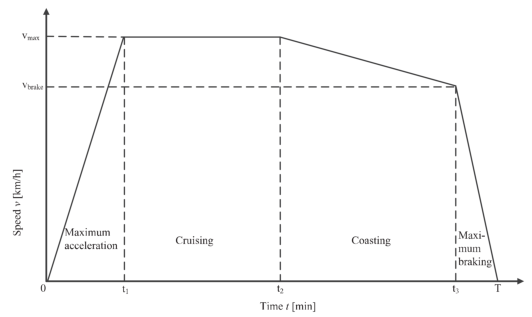
\includegraphics[width=0.5\textwidth,keepaspectratio]{figures/35.DSS/scheepmaker2017a}
%			\caption{Optimal traction regimes. Adapted from \cite{scheepmaker2017}.}
%		\end{figure}
		
%	\end{minipage}

%\end{block}
%\end{frame}
%%%%%%%%%%%%%%%%%%%%%%%%%%%%%%%%%%%%%%%%%%%%%%%%%%%%%%%%%%%%%%%%%%%%%%%%%%%%%%%%%%%%%

%\subsection{Issues and problems in Wireless Networks}
%%%%%%%%%%%%%%%%%%%%%%%%%%%%%%%%%%%%%%%%%%%%%%%%%%%%%%%%%%%%%%%%%%%%%%%%%%%%%%%%%%%%%

\begin{frame}{Literature review}{Outline}
	\begin{block}{\textbf{Literature Review}}
		\begin{itemize}
			\item Power System of Railway Transportation System
			\item Energy Sensors
			\item Wireless Networks
			\item Smart Metering
			\item \textbf{Decision Support Systems}
			\item \textbf{Issues and Problems in WSN --- Outliers}
		\end{itemize}
	\end{block}
\end{frame}



%\begin{frame}{Issues and problems in Wireless Networks}{Outlier Detection Techniques}
%\begin{block}{\textbf{Outlier Detection Techniques for RTS}}
	
%	\begin{minipage}[t]{0.6\linewidth}
		%	\vspace{5em}
%		\begin{itemize}
			%\setlength\itemsep{-0.5em}
%			\footnotesize
%			\item \textbf{Classification based techniques.}
%			\begin{itemize}
%				\item Bayesian Networks
%				\item Rule-based techniques
%				\item Support Vector Machines
%			\end{itemize}
			
%			\item \textbf{Statistical based techniques.}
%			\begin{itemize}
%				\item Parametric --- Gaussian based
%				\item Non-parametric --- Histogram based
%				\item Non-parametric --- Kernel function based
%			\end{itemize}
		
%			\item \textbf{Nearest Neighbor-based techniques.}
%			\begin{itemize}
%				\item Using distance
%				\item Using relative density
%			\end{itemize}
%			\item \textbf{Clustering based techniques.}
			
%			\item \textbf{Spectral Decomposition based techniques.}
			
%		\end{itemize}
%	\end{minipage}\hfill
%	\begin{minipage}[t]{0.38\linewidth}
		
%		\begin{figure}[ht!]
%			\centering
%			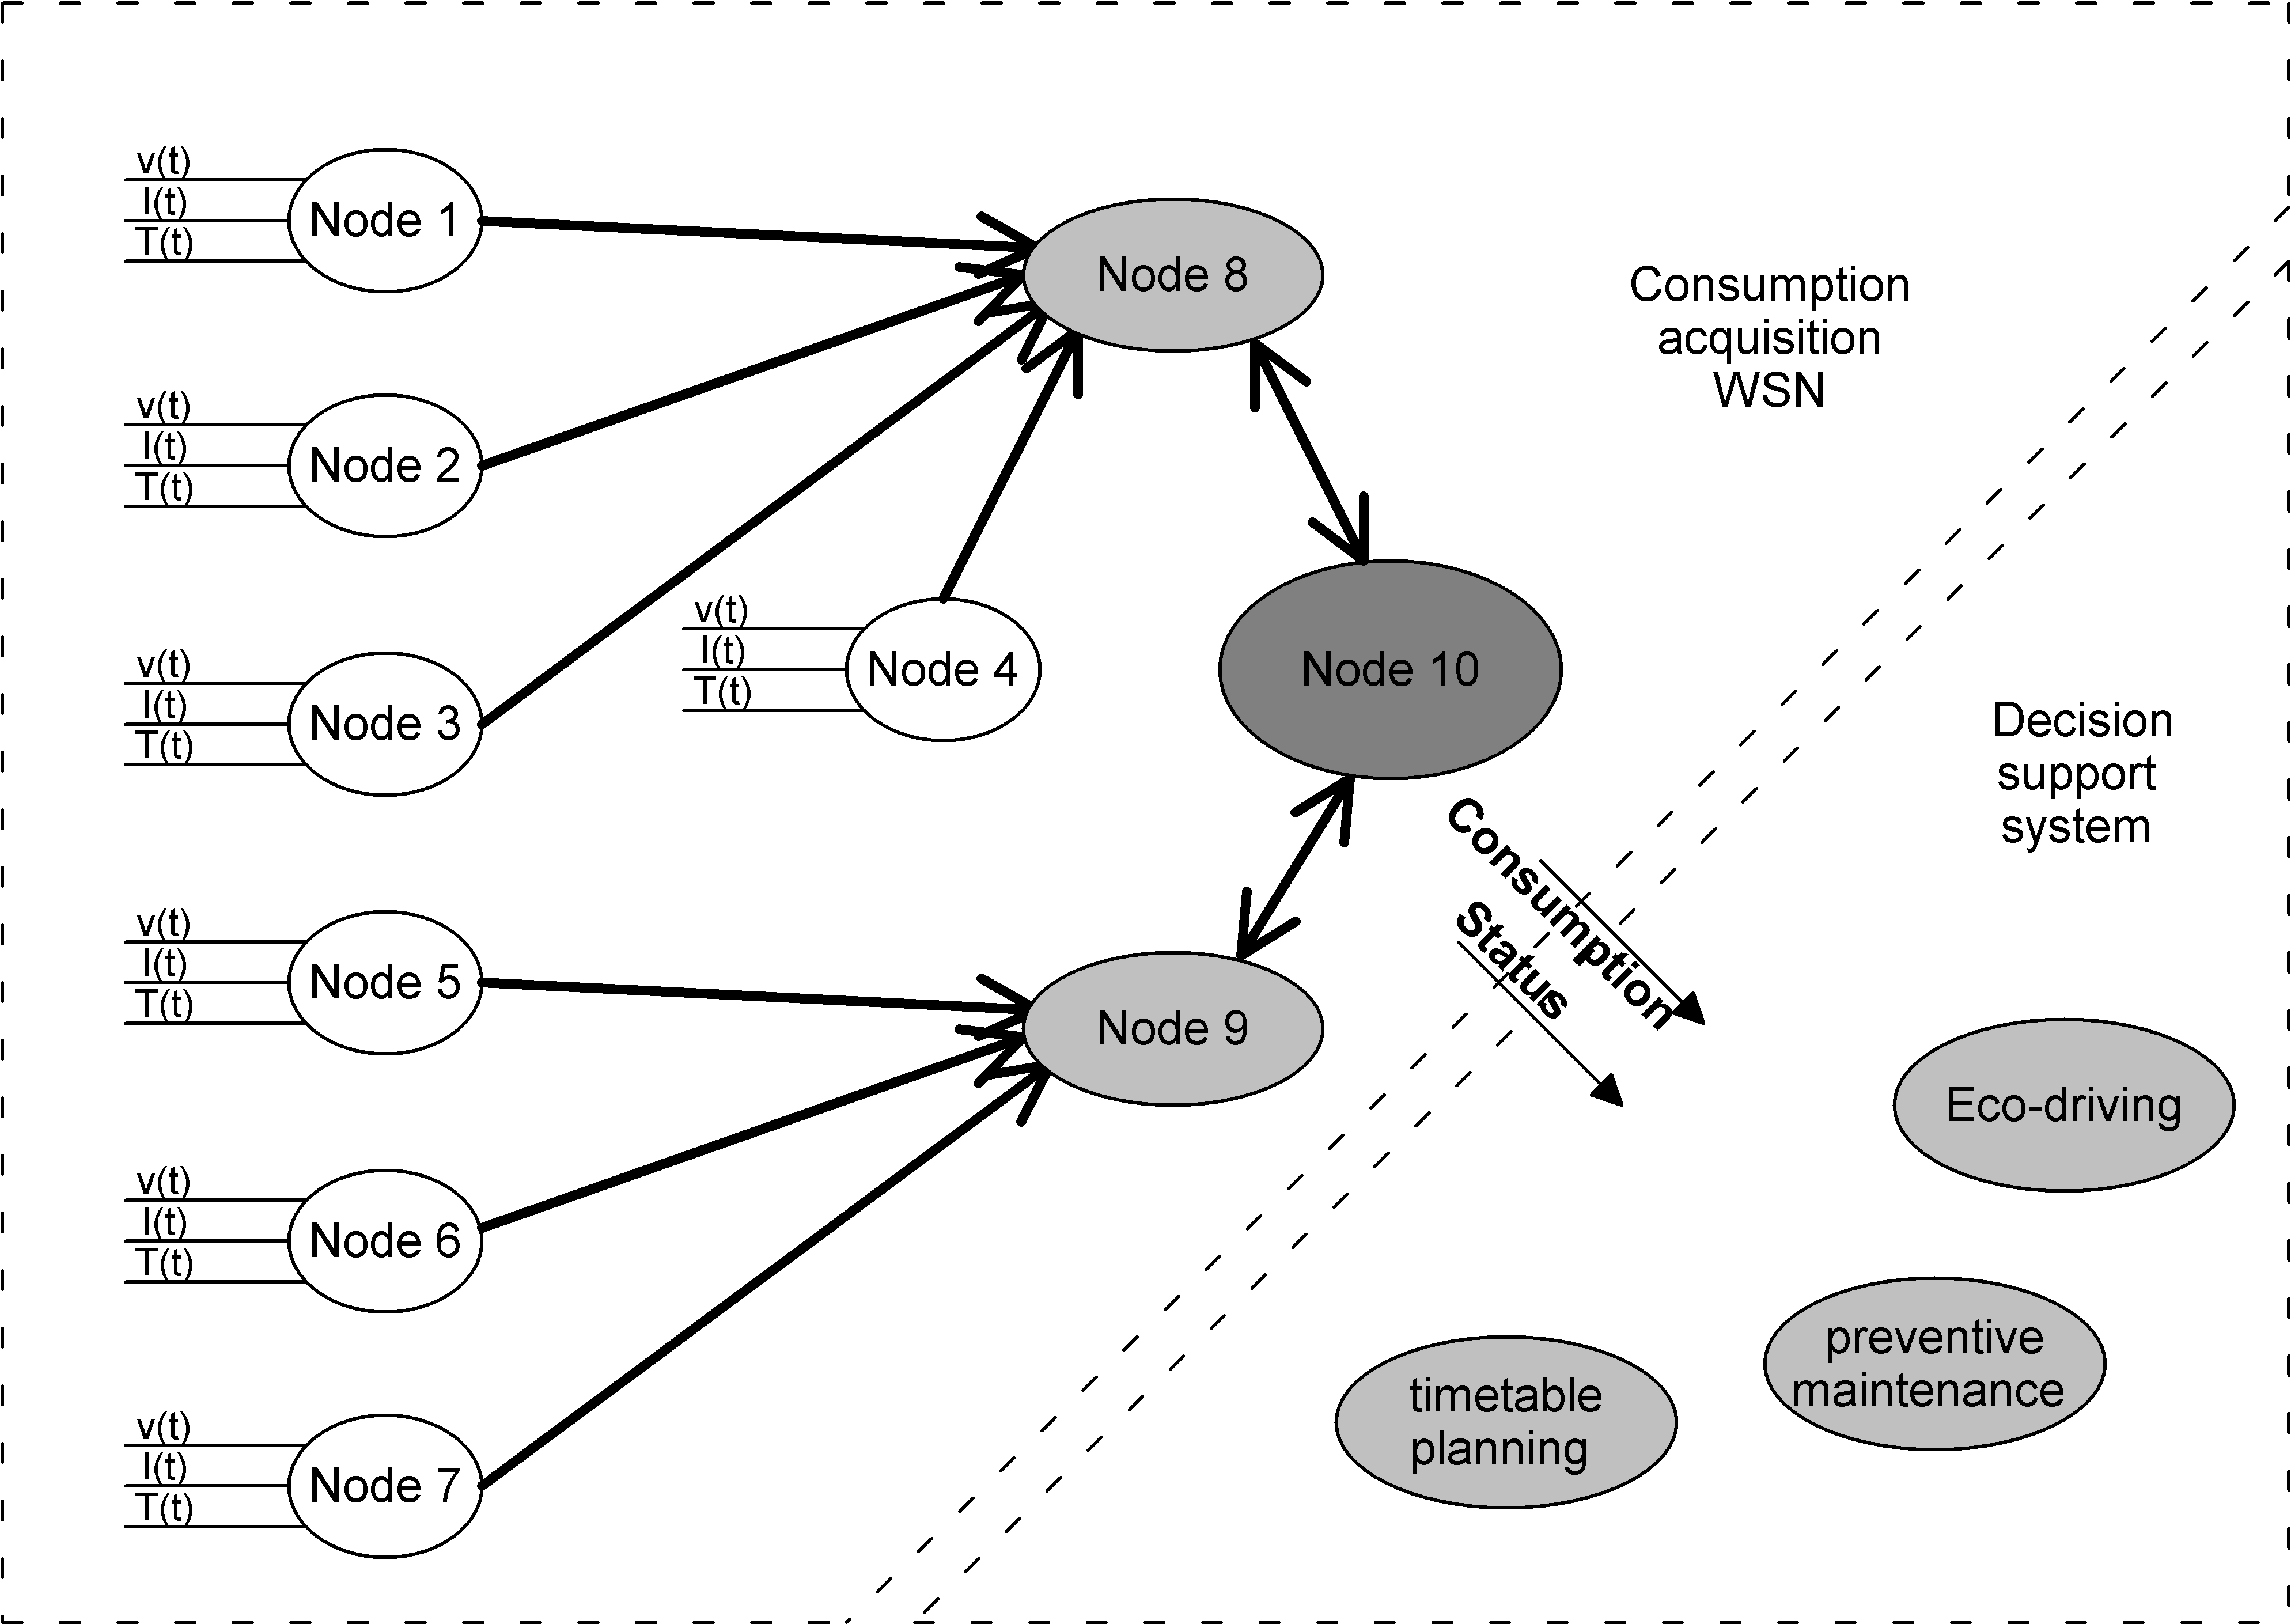
\includegraphics[width=0.95\textwidth,keepaspectratio]{figures/36.Outlier/general}
%			\caption{Integration of the \ac{WSN} with a decision support system. }
%		\end{figure}
		
%	\end{minipage}
	
%\end{block}
%\end{frame}

%%%%%%%%%%%%%%%%%%%%%%%%%%%%%%%%%%%%%%%%%%%%%%%%%%%%%%%%%%%%%%%%%%%%%%%%%%%%%%%%%%%%%